\subsection{Badania wpływu parametrów adaptacyjnych na uczenie sieci}
Na podstawie wyników poprzednich eksperymentów ustalono konfigurację sieci na 70 neuronów w warstwie pierwszej i 13 w warstwie drugiej. Współczynnik uczenia ustawiono na 0.01. Pozostałe współczynniki zmieniano w zagnieżdżonych pętlach. Współczynnik zwiększania wartości współczynnika uczenia $lr\_inc$ zmieniano w zakresie od 1.03 do 1.07 z krokiem 0.01, współczynnik $lr\_dec$ w zakresie od 0.6 do 0.8 z krokiem 0.05, oraz dopuszczalna krotność przyrostu błędu (w Matlab'ie $max\_perf\_inc$) w zakresie od 1.02 do 1.06 z krokiem 0.01.

\begin{figure}[!htb]
\minipage{0.5\textwidth}
  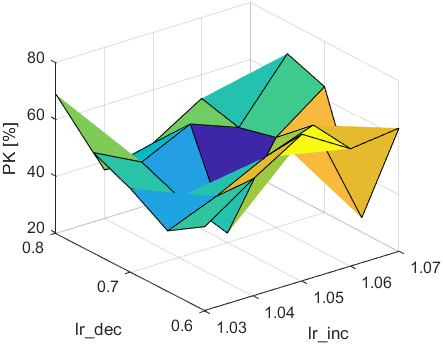
\includegraphics[width = \linewidth]{Grafika/exp5/pk102.png}
\endminipage\hfill
\minipage{0.5\textwidth}
  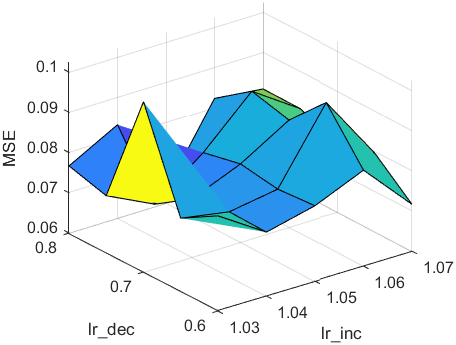
\includegraphics[width = \linewidth]{Grafika/exp5/mse102.png}
\endminipage\hfill
\caption{Wpływ $lr\_inc$ i $lr\_dec$ na $PK$ i $MSE$ dla $max\_perf\_inc=1.02$}
\end{figure}
%\\[0.5cm]
\begin{figure}[!htb]
\minipage{0.5\textwidth}
  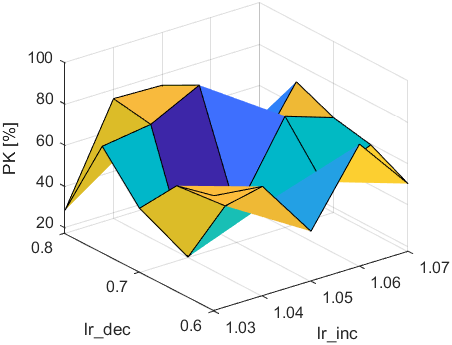
\includegraphics[width = \linewidth]{Grafika/exp5/pk103.png}
\endminipage\hfill
\minipage{0.5\textwidth}
  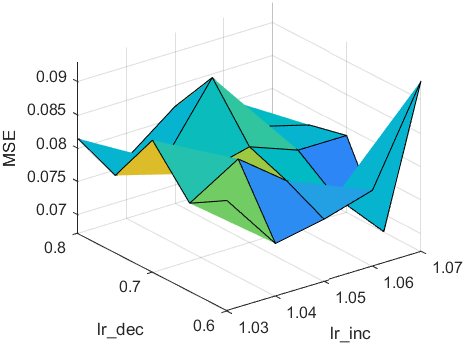
\includegraphics[width = \linewidth]{Grafika/exp5/mse103.png}
\endminipage\hfill
\caption{Wpływ $lr\_inc$ i $lr\_dec$ na $PK$ i $MSE$ dla $max\_perf\_inc=1.03$}
\end{figure}

\clearpage
\begin{figure}[!htb]
\minipage{0.5\textwidth}
  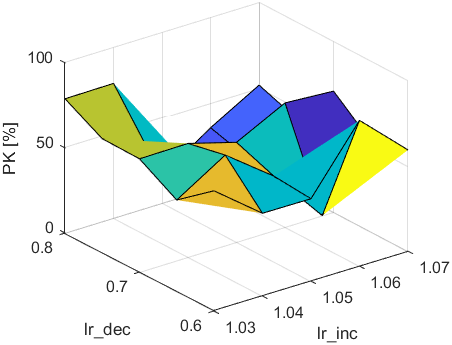
\includegraphics[width = \linewidth]{Grafika/exp5/pk104.png}
\endminipage\hfill
\minipage{0.5\textwidth}
  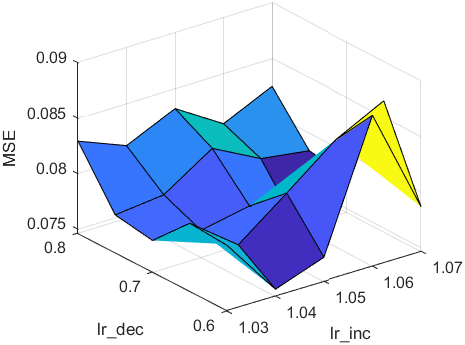
\includegraphics[width = \linewidth]{Grafika/exp5/mse104.png}
\endminipage\hfill
\caption{Wpływ $lr\_inc$ i $lr\_dec$ na $PK$ i $MSE$ dla $max\_perf\_inc=1.04$}
\end{figure}

\begin{figure}[!htb]
\minipage{0.5\textwidth}
  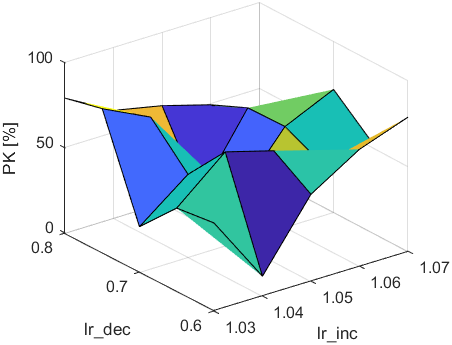
\includegraphics[width = \linewidth]{Grafika/exp5/pk105.png}
\endminipage\hfill
\minipage{0.5\textwidth}
  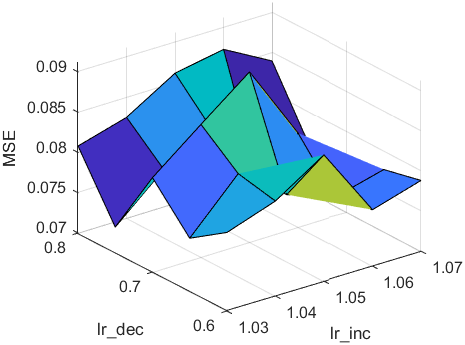
\includegraphics[width = \linewidth]{Grafika/exp5/mse105.png}
\endminipage\hfill
\caption{Wpływ $lr\_inc$ i $lr\_dec$ na $PK$ i $MSE$ dla $max\_perf\_inc=1.05$}
\end{figure}
\begin{figure}[!htb]
\minipage{0.5\textwidth}
  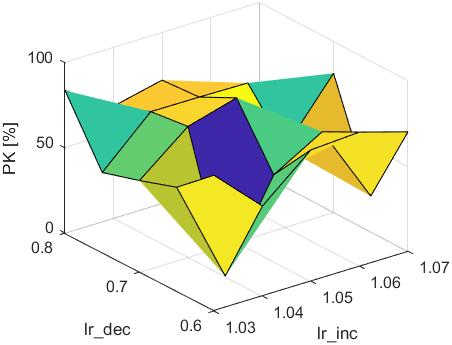
\includegraphics[width = \linewidth]{Grafika/exp5/pk106.png}
\endminipage\hfill
\minipage{0.5\textwidth}
  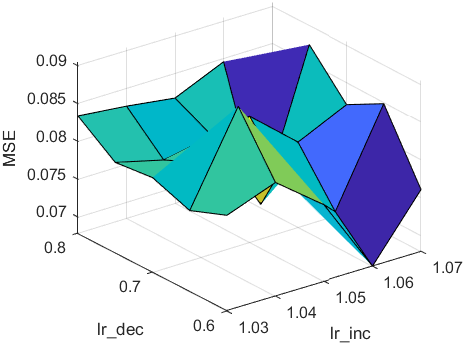
\includegraphics[width = \linewidth]{Grafika/exp5/mse106.png}
\endminipage\hfill
\caption{Wpływ $lr\_inc$ i $lr\_dec$ na $PK$ i $MSE$ dla $max\_perf\_inc=1.06$}
\end{figure}

Największą poprawność klasyfikacji ($85.63\%$) uzyskano dla $lr\_inc = 1.06$, $lr\_dec = 0.6$ i $max\_perf\_inc=1.04$. Błąd średnio kwadratowy dla tej konfiguracji wynosił $0.0882536$.